\chapter{Pontos de Interesse}\label{sec:pontosdeinteresse}
%======================================================================================
%
A reconstrução 3D pelo método da estrutura do movimento, ou {\it Structure from Motion} ({\it SfM}). Tem como base a utilização de pontos de interesse
({\it features}), que são pontos ou áreas em comum entre as imagens usadas na reconstrução. Para encontrar estes pontos, diferentes algoritmos são empregados.

\section { SIFT -- {\it Scale Invariant Feature Transform}}

Primeiramente, utiliza-se o SIFT (algoritmo de detecção de pontos de interesse, invariante à escala e à transformações, como rotação, translação e iluminação da imagem, por exemplo).
O algoritmo pode ser dividido em cinco etapas, das quais:

\begin{itemize}
	\item{Deteccão de espaço-escala extremos -- {\it Scale-space Extrema Detection}}
	\item{Localização de pontos-chaves -- {\it Keypoint Localization}}
	\item{Atribuição de orientação -- {\it Orientation Assignment}}
	\item{Descritor de pontos-chaves -- {\it Keypoint Descriptor}}
	\item{Combinação de pontos-chaves -- {\it Keypoint Matching}}
\end{itemize}


\subsection{Detecção de espaço-escala extremos}

% From the image above, it is obvious that we can't use the same window to detect keypoints with different scale. It is OK with small corner. But to detect larger corners we need larger windows. For this, scale-space filtering is used. In it, Laplacian of Gaussian is found for the image with various σ values. LoG acts as a blob detector which detects blobs in various sizes due to change in σ. In short, σ acts as a scaling parameter. For eg, in the above image, gaussian kernel with low σ gives high value for small corner while guassian kernel with high σ fits well for larger corner. So, we can find the local maxima across the scale and space which gives us a list of (x,y,σ) values which means there is a potential keypoint at (x,y) at σ scale.

Em casos com cantos pequenos, a detecção funciona bem. Porém, raramente utilizaremos a mesma janela para detectar pontos-chaves em imagens com diferentes escalas, pois utilizamos imagens grandes e, consequentemente, cantos grandes. Para isso, precisamos de janelas grandes também. 

Para resolver este problema, o filtro de escala-espaço é usado: o Laplaciano de Gaussiano ({\it Laplacian of Gaussian} --  LoG). O LoG atua como um detector de particulas em diferentes tamanhos $\sigma$. (Onde $\sigma$ é o parâmetro de escala). Por exemplo, o núcleo gaussiano com $\sigma$ baixo, tem como resposta um alto valor para um canto pequeno. Enquanto um núcleo gaussiano com alto $\sigma$, se encaixa bem para um canto maior. Com esta lógica, podemos encontrar um máximo local através da escala e o espaço, o que nos fornece uma lista de $(x,y \sigma)$, o que significa que existe um ponto-chave em potencial, com o par $(x,y)$ na escala $\sigma$.

% \begin{equation}
% LoG(x,y) = - \frac{1}{\pi \sigma ^4 }\left [ 1 - \frac{x^2+y^2}{2 \sigma ^2} \right ]e^{- \frac{x^2+y^2}{2 \sigma ^2}} 
% \end{equation}

Porém, como o LoG é um pouco custoso, computacionalmente. O SIFT utiliza um algoritmo aproximado do LoG, o DoG (Diferença de Gaussianos -- {\it Difference of Gaussians}). O DoG é a diferença de um filtro Gaussiano de uma imagem, com dois valores diferentes de escala $\sigma$. 

Uma aplicação prática do filtro DoG é a sequência de imagens a seguir:

\begin{figure} [!h]
	\centering
	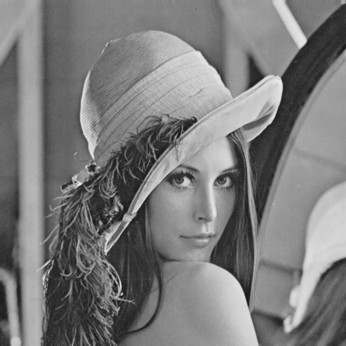
\includegraphics[width=0.45\linewidth]{figs/lena.jpg}(a)
	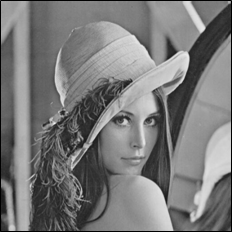
\includegraphics[width=0.45\linewidth]{figs/lenaSigma1.png}(b)
	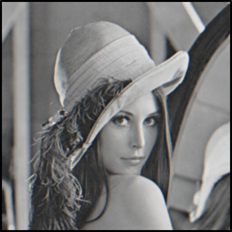
\includegraphics[width=0.45\linewidth]{figs/lenaSigma2.png}(c)
 	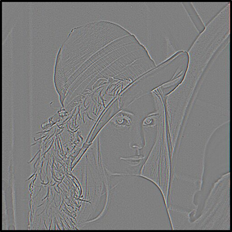
\includegraphics[width=0.45\linewidth]{figs/lenaDoG.png} (d)
	\caption{%
	É aplicado um filtro gaussiano na imagem original (a), com $\sigma$ = 1, tendo como resultado a imagem (b).
	Um outro filtro gaussiano é usado, porém, neste caso, o $\sigma$ = 2 (c). Após isso, subtrai-se (b) de (c), obtendo 
	o filtro DoG (d).
	}\label{fig:lenadog}
\end{figure}

Uma vez que o DoG é aplicado, as iamgens são utilizadas com o espaço e escala extremos. Por exemplo, na imagem \ref{fig:extrema}, um pixel é comparado com seus 8 vizinhos, assim como comparado com os 9 pixels na próxima escala e os 9 pixels na escala anterior. Se esse pixel é um local extremo, ele é um ponto-chave em potencial. Isto é, este ponto-chave é melhor representado nesta escala.

\begin{figure}
	\centering
	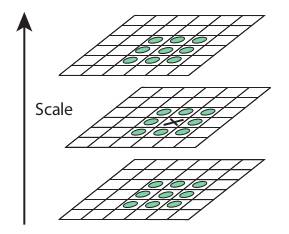
\includegraphics[width=0.45\linewidth]{figs/sift_local_extrema.jpg}
	\caption{%
	Exemplo de funcionamento de deteccão de espaço-escala extrema
	}\label{fig:extrema}
\end{figure}

No caso, as funções ficariam da seguinte forma: 

\begin{equation}
\label{eq:gaussiano}
	g_\sigma(x) = \frac{1}{2 \pi \sigma ^2} e^{-\frac{1}{2} \frac{x^T x}{\sigma ^2}}
\end{equation}

\begin{equation}
\label{eq:gaussianScaleSpace}
	I_\sigma = g_\sigma * I, \sigma >= 0
\end{equation}

\begin{equation}
\label{eq:LoG}
	\triangledown^2	g_\sigma(x)
\end{equation}

\begin{equation}
\label{eq:DoG}
	DoG_\sigma(o,s) = I_\sigma(o,s+1) - I_\sigma(o,s)
\end{equation}


Onde \ref{eq:gaussiano} é a função padrão do operador gaussiano (núcleo), a equação \ref{eq:LoG} é o operador LoG,  \ref{eq:DoG} é o operador DoG e $\triangledown^2$ é o operador Laplaciano.

\subsection{Localização de pontos-chaves}

A localização dos pontos extremos pode cair em um extremo local e não global. Logo, após a utilização do DoG e com os pontos-chaves em potencial localizados, eles precisam ser refinados para melhorar o resultado. Para isso, são utilizadas Séries de Taylor na escala e no espaço, e, se a intensidade nesse extremo é menor que o valor limite, este é rejeitado.
%TODO: Ver isso 
Os {\it frames} do SIFT (pontos-chaves) são extraídos baseados nos extremos locais (picos) a partir do DoG. Numericamente, extremos locais são elementos que possuem um menor (ou maior) valor em uma vizinhança em um espaço 3x3x3 (em escala e espaço).
Depois de extraídos, estes pontos são interpolados quadraticamente (este passo é muito importante, especialmente nas escalas de menor resolução, para ter uma localização precisa do ponto-chave na resolução completa). Finalmente, eles são filtrados para eliminar respostas de baixo contraste ou respostas próximas as bordas.

%Eliminating low contrast responses

Picos que são pequenos, na maior parte das vezes são gerados a partir de ruídos e necessitam ser descartados também. Isso é feito com uma comparação de valor absoluto do DoG no pico com o valor do pico limite e é descartado caso este valor é menor que o limite.


%Eliminating edge responses 

Para eliminar respostas em bordas, normalmente os picos mais rasos ou horizontais, são gerados por bordas e não possuem características estáveis, portanto estes picos precisam ser removidos. Para isso, dado um pico (x, y, $\sigma$), o algoritmo avalia a matriz Hessiana (x,y) do DoG na escala $\sigma$. Então é computado um valor para esta equação (\ref{eq:hessianaDoG}):

\begin{equation}
	v = \frac{( T_r \ D(x,y,\sigma))^2}{Det \ D(x,y,\sigma)}
	\label{eq:hessianaDoG}
\end{equation}
Onde, $T_r$ é o traço, ou seja, $T_r(H) = D_{xx} + D_{yy}$ e a matriz $D$ é do tipo
\[D = \begin{bmatrix}
	\frac{\partial ^2 DoG}{\partial x^2} & \frac{\partial ^2 DoG}{\partial x \partial y} \\ 
	\frac{\partial ^2 DoG}{\partial x \partial y} & \frac{\partial ^2 DoG}{\partial y^2} 
\end{bmatrix}
\]

No caso, v possui um valor mínimo (igual a 4) quando os autovalores da Jacobiana são iguais (pico curvado) e aumentam à medida que um dos autovalores aumenta e os outros permanecem baixos. Os picos são retidos se $v  < \frac{(t_e+1)(t_e+1)}{t_e}$ , onde $t_e$ é o limite da borda. 

\subsection{Atribuição de orientação}

Agora, uma orientação é atribuída a cada ponto-chave para obter a invariância à rotação da imagem. 
Uma vizinhança é obtida, dependente da escala, do gradiente da magnitude \ref{eq:magnitudeSIFT} e da direção \ref{eq:direcaoSIFT} (usando diferenças finitas), ao redor da localização do ponto-chave. 

\begin{equation}
	m(x,y) = \sqrt{(L(x+1,y)-L(x-1,y))^2 + (L(x,y+1)-L(x,y-1)^2)}
	\label{eq:magnitudeSIFT}
\end{equation}

\begin{equation}
	\theta = tan^{-1} \left( \frac{(L(x,y+1)-L(x,y-1)}{(L(x+1,y)-L(x-1,y)}\right)
	\label{eq:direcaoSIFT}
\end{equation}

Então, um histograma de 36 orientações ({\it bins}) cobrindo 360 graus é criado. Onde ele é ponderado pelo gradiente da magnitude e por uma janela Gaussiana circular onde $\sigma$ vale $1.5$ em relação à escala do ponto-chave \ref{fig:histogramaOrientado}.

\begin{figure} [!h]
	\centering
	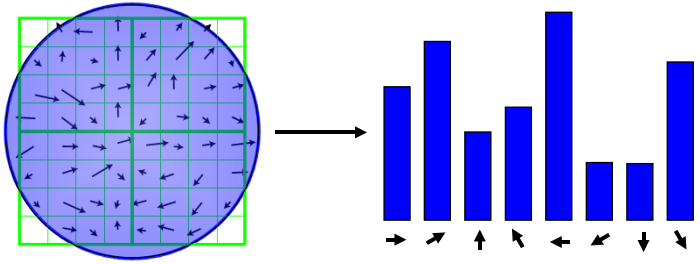
\includegraphics[width=0.45\linewidth]{figs/histogramaOrientado.png}
	\caption{%
	Exemplo do resultado obtido do histograma orientado
	}\label{fig:histogramaOrientado}
\end{figure}

O ponto mais do histograma é obtido e qualquer pico acima de 80\% é considerado no cálculo da orientação. 
Pontos-chaves são criados com a mesma localização e escala, mas em diferentes direções, o que contribui para a establidade da correspondência.

\subsection{Descritor de pontos-chaves}

Com os pontos-chaves criados a partir do histograma orientado, cria-se agora o descritor de pontos-chaves.

Uma vizinhança 16x16 ao redor do ponto-chave é escolhida e esta mesma vizinhaça é dividida em 16 sub-blocos 4x4. Para cada bloco, um histograma orientado com 8 {\it bin} é criado. Logo, temos 128 valores válidos de {\it bin}. Esses valores são representados em forma de vetor para expressar o descritor de pontos-chaves \ref{fig:descritorKeypoint}. 

Além disso, são tomadas algumas medidas para deixar o descritor mais robusto,como, por exemplo, invariante à luminosidade, rotação, etc.

\begin{figure} [!h]
	\centering
	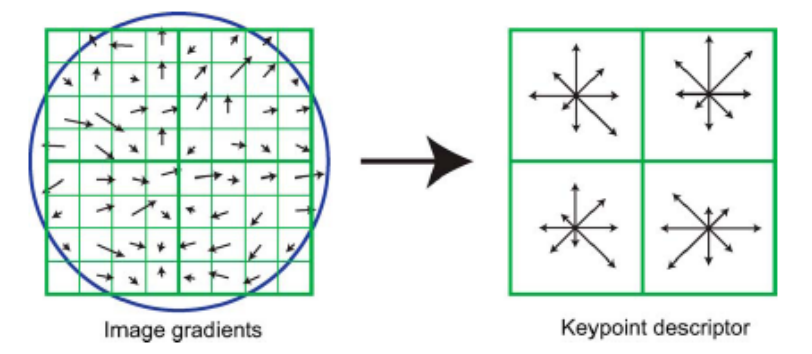
\includegraphics[width=0.45\linewidth]{figs/descritorKeypoint.png}
	\caption{%
	Exemplo de um descritor de pontos-chaves, com uma matriz 2x2 e uma região 8x8
	}\label{fig:descritorKeypoint}
\end{figure}

\subsection{Combinação de pontos-chaves}

Pontos-chaves entre duas imagens são combinados a partir da identificação da vizinhança mais próxima. Mas, em alguns casos, a segunda combinação mais próxima pode ser parecida com a primeira. Isso se dá por ruídos presentes nas imagens ou algo assim. 

Nesse caso, a razão da distância mais próxima para a segunda distância mais próxima é utilizada. Se essa razão for maior que 0.8, essa combinação é descartada.
Esse método elimina cerca de 90\% de combinações falsas, enquanto descarta apenas cerca de 5\% de combinações corretas.

\section {Triangulação -- {\it Full pairwise image matching}}